% Copyright 2020-2023 Robert Bosch GmbH

% Licensed under the Apache License, Version 2.0 (the "License");
% you may not use this file except in compliance with the License.
% You may obtain a copy of the License at

% http://www.apache.org/licenses/LICENSE-2.0

% Unless required by applicable law or agreed to in writing, software
% distributed under the License is distributed on an "AS IS" BASIS,
% WITHOUT WARRANTIES OR CONDITIONS OF ANY KIND, either express or implied.
% See the License for the specific language governing permissions and
% limitations under the License.

The \pkg\ is a command-line utility designed to streamline issue synchronization 
across various tracking systems, including \textbf{GitHub}, \textbf{Jira}, 
\textbf{GitLab} and \textbf{IBM RTC}. 

Its primary objective is to automate and simplify the integration and 
synchronization of issues between these platforms, enabling efficient tracking 
and planning for teams that work with multiple tools.

\begin{figure}[h!]
   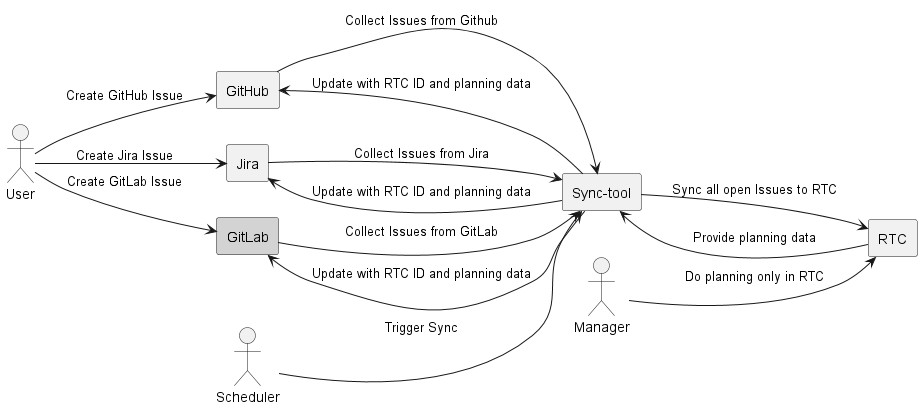
\includegraphics[width=1\linewidth]{./pictures/usecase_diagram.png}
   \caption{Tool's use case}
\end{figure}

\section{Use Cases}

\begin{itemize}
    \item \textbf{Multi-Tool Teams:} For teams using a combination of GitHub, 
          Jira, and RTC for issue management, this tool acts as a bridge to 
          consolidate data.
    \item \textbf{Planning and Reporting:} Synchronization ensures managers and 
          stakeholders have a centralized view of issues for effective planning.
    \item \textbf{Automated Workflows:} With scheduled triggers, the tool 
          eliminates manual synchronization efforts, saving time and reducing 
          errors.
\end{itemize}

\section{Benefits}

\begin{itemize}
    \item \textbf{Automation:} Reduces manual synchronization overhead.
    \item \textbf{Consistency:} Ensures data integrity across platforms.
    \item \textbf{Customizable:} Flexible configurations to suit various project 
          needs.
    \item \textbf{Centralized Planning:} Aligns all issues with RTC, the central 
          planning tool.
\end{itemize}